% Make nice A4 pages for print:
%\usepackage{pgfpages}
%\pgfpagesuselayout{resize to}[a4paper,border shrink=5mm,landscape]

\beamertemplatenavigationsymbolsempty

\setbeamertemplate{bibliography item}[text]

\usepackage[type={CC},modifier={by-sa},version={4.0}]{doclicense}

\usepackage[utf8]{inputenc}
\usepackage{hyperref}
\usepackage{breakurl}
\usepackage{graphicx}
\usepackage{pgfplots}
\usepackage{pgf}
\usepackage{tikz}
\usetikzlibrary{positioning}
\usetikzlibrary{arrows}
\usetikzlibrary{decorations.markings}
\usetikzlibrary{calc}
\usetikzlibrary{matrix}
\usetikzlibrary{shapes}
\usetikzlibrary{decorations.pathmorphing}
\usetikzlibrary{fit}
\usetikzlibrary{backgrounds}
\usetikzlibrary{plotmarks}
\usepackage{stmaryrd}
\usepackage{listings}
\usepackage{pdflscape}
\usepackage{perpage}
\usepackage{appendixnumberbeamer}

%\usepackage[thmmarks,amsmath,amsthm]{ntheorem} % already included in beamer
\usepackage{thm-restate}

\usepackage[sort&compress,numbers]{natbib}  % to be have \citet, \citeauthor, \citeyear

\MakePerPage{footnote}

\tikzstyle{o}=[r,ppBlue]
\tikzstyle{r}=[thick,rectangle,align=center]
\tikzstyle{t}=[r,ppTrans] %,font=\bfseries]
\tikzstyle{dd}=[densely dashed]
\tikzstyle{n}=[r,ppBlue]
\tikzstyle{p}=[r,ppRed]
\tikzstyle{ppRed}  =[draw=red,  fill=  red!20]
\tikzstyle{ppBlue} =[draw=blue, fill= blue!20]
\tikzstyle{ppGreen}=[draw=green,fill=green!20]
\tikzstyle{ppTrans}=[draw=none, fill=none]

\usetheme{Warsaw}

\useoutertheme[subsection=true]{smoothbars}
%\useoutertheme[subsection=false]{miniframes}

\definecolor{bblue}{HTML}{D7DF01}	% yellow-ish actually, for better black/white printing
\definecolor{rred}{HTML}{C0504D}
\definecolor{ggreen}{HTML}{9BBB59}
\definecolor{ppurple}{HTML}{9F4C7C}
\definecolor{lightgray}{rgb}{0.3,0.3,0.3}
\definecolor{lightergray}{rgb}{0.9,0.9,0.9}
\definecolor{UniBlue}{RGB}{83,121,170}

\DeclareTextFontCommand\textintro{\normalfont\bfseries\itshape} % nice!
\newcommand{\intro}[2][]
{%
	\textintro{#2}%
}
\newcommand{\empha}[2][]
{%
	\emph{#2}%
}

%\theoremstyle{plain}
\newcounter{reqcounter}
\newtheorem{requirement}[reqcounter]{Requirement}

%setbeamercolor{structure}{fg=violet}

\makeatletter
\def\th@task{%
    \normalfont % body font
    \setbeamercolor{block title example}{bg=orange,fg=white}
    \setbeamercolor{block body example}{bg=orange!20,fg=black}
    \def\inserttheoremblockenv{exampleblock}
  }
\makeatother

\theoremstyle{task}
\newtheorem{task}{Task}

\newenvironment{assignment}%
{%\setbeamercolor{background canvas}{bg=violet}%
%\setbeamercolor{structure}{fg=cyan!90!black}%
 \setbeamercolor{frametitle}{bg=orange,fg=white}
\begin{frame}}%
{\end{frame}}%

\AtBeginSection[]{
  \begin{frame}
  \vfill
  \centering
  \begin{beamercolorbox}[sep=8pt,center,shadow=true,rounded=true]{title}
    \usebeamerfont{title}\insertsectionhead\par%
  \end{beamercolorbox}
  \tableofcontents
  \vfill
  \end{frame}
}




\pgfplotsset{compat=1.14}
\author{Markus Raab}


\date{29.01.2020}

\begin{document}

\renewcommand{\enquote}[1]{\emph{``#1''}} % Cannot be done earlier

%%%%%%%%%%%%%%%%%%%%%%%%%%%%%%%
\begin{frame}
	\titlepage
	\doclicenseThis
\end{frame}




%%%%%%%%%%%%%%%%%%%%%%%%%%%%%%%%%%%%%%%%%% 
\section{Elektra}

\subsection{Basics}

\begin{frame}
	\frametitle{Elektra as Virtual Filesystem}
	\begin{itemize}
	\item configuration files are seen like ``block devices''
	\item are mounted with respective filesystem drivers into the filesystem
	\item many tools and APIs evolved to work with files
	\item Idea of Elektra: establish a similar ecosystem for configuration
	\end{itemize}
\end{frame}

\begin{frame}
	\frametitle{Why is Elektra not a Filesystem then?}
	\begin{itemize}
	\item API semantics: key/value get/set
	\item namespaces: based on established semantics
	\item many features essential for misconfiguration hardening:
		\begin{itemize}
		\item validation
		\item visibility
		\item defaults
		\item \dots (extensible specification)
		\end{itemize}
	\end{itemize}
\end{frame}

% hack: needed to render graphics properly
\begin{frame}<0>[noframenumbering]
	\begin{columns}[c]
	\begin{column}{7cm}
	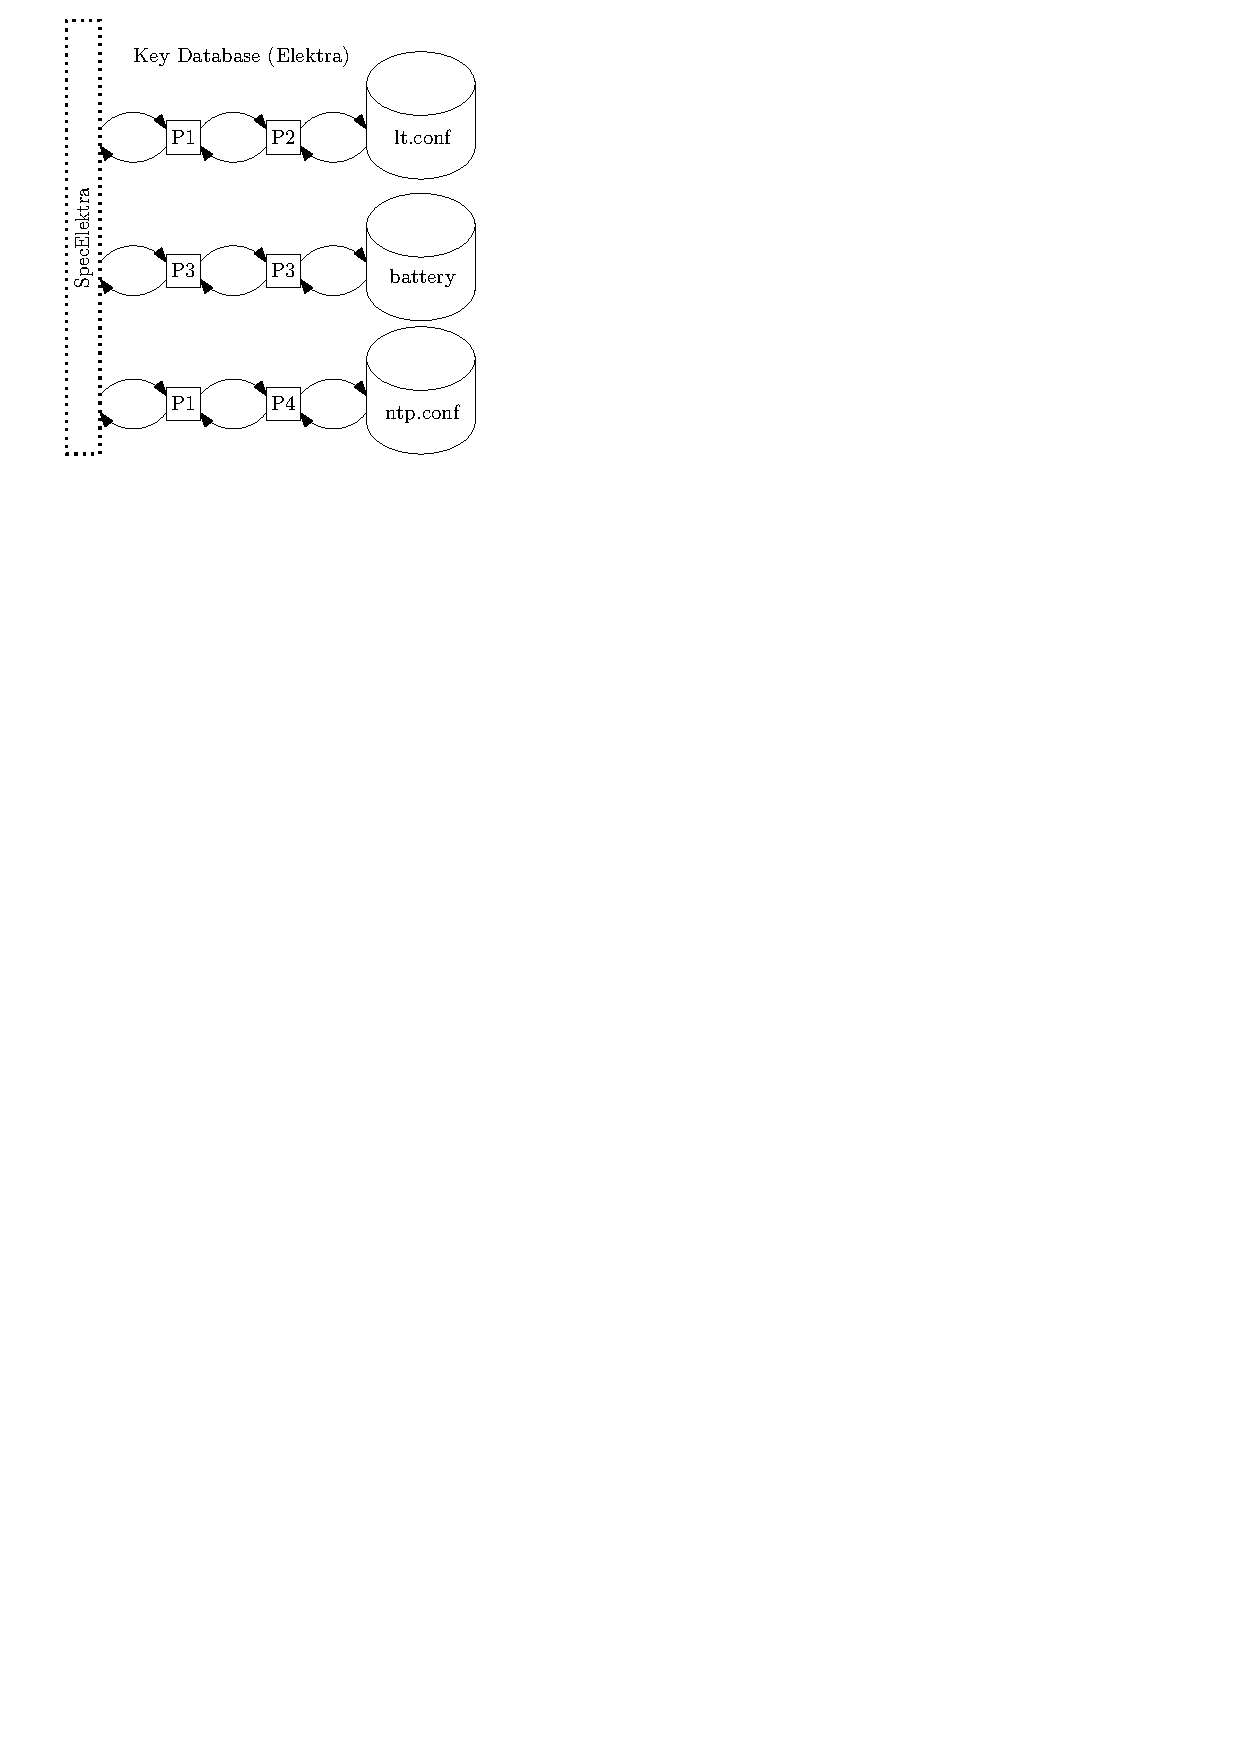
\includegraphics[scale=0.8]{horizontalmodularity}
	\end{column}
	\begin{column}{4cm}
	Cylinders are configuration files, P? are plugins~\cite{raab2016improving}.

	Key ideas:
	\begin{itemize}
	\item all work is done by plugins
	\item central data structure implements semantics
	\end{itemize}
	\end{column}
	\end{columns}
\end{frame}

\begin{frame}
	\begin{columns}[c]
	\begin{column}{7cm}
	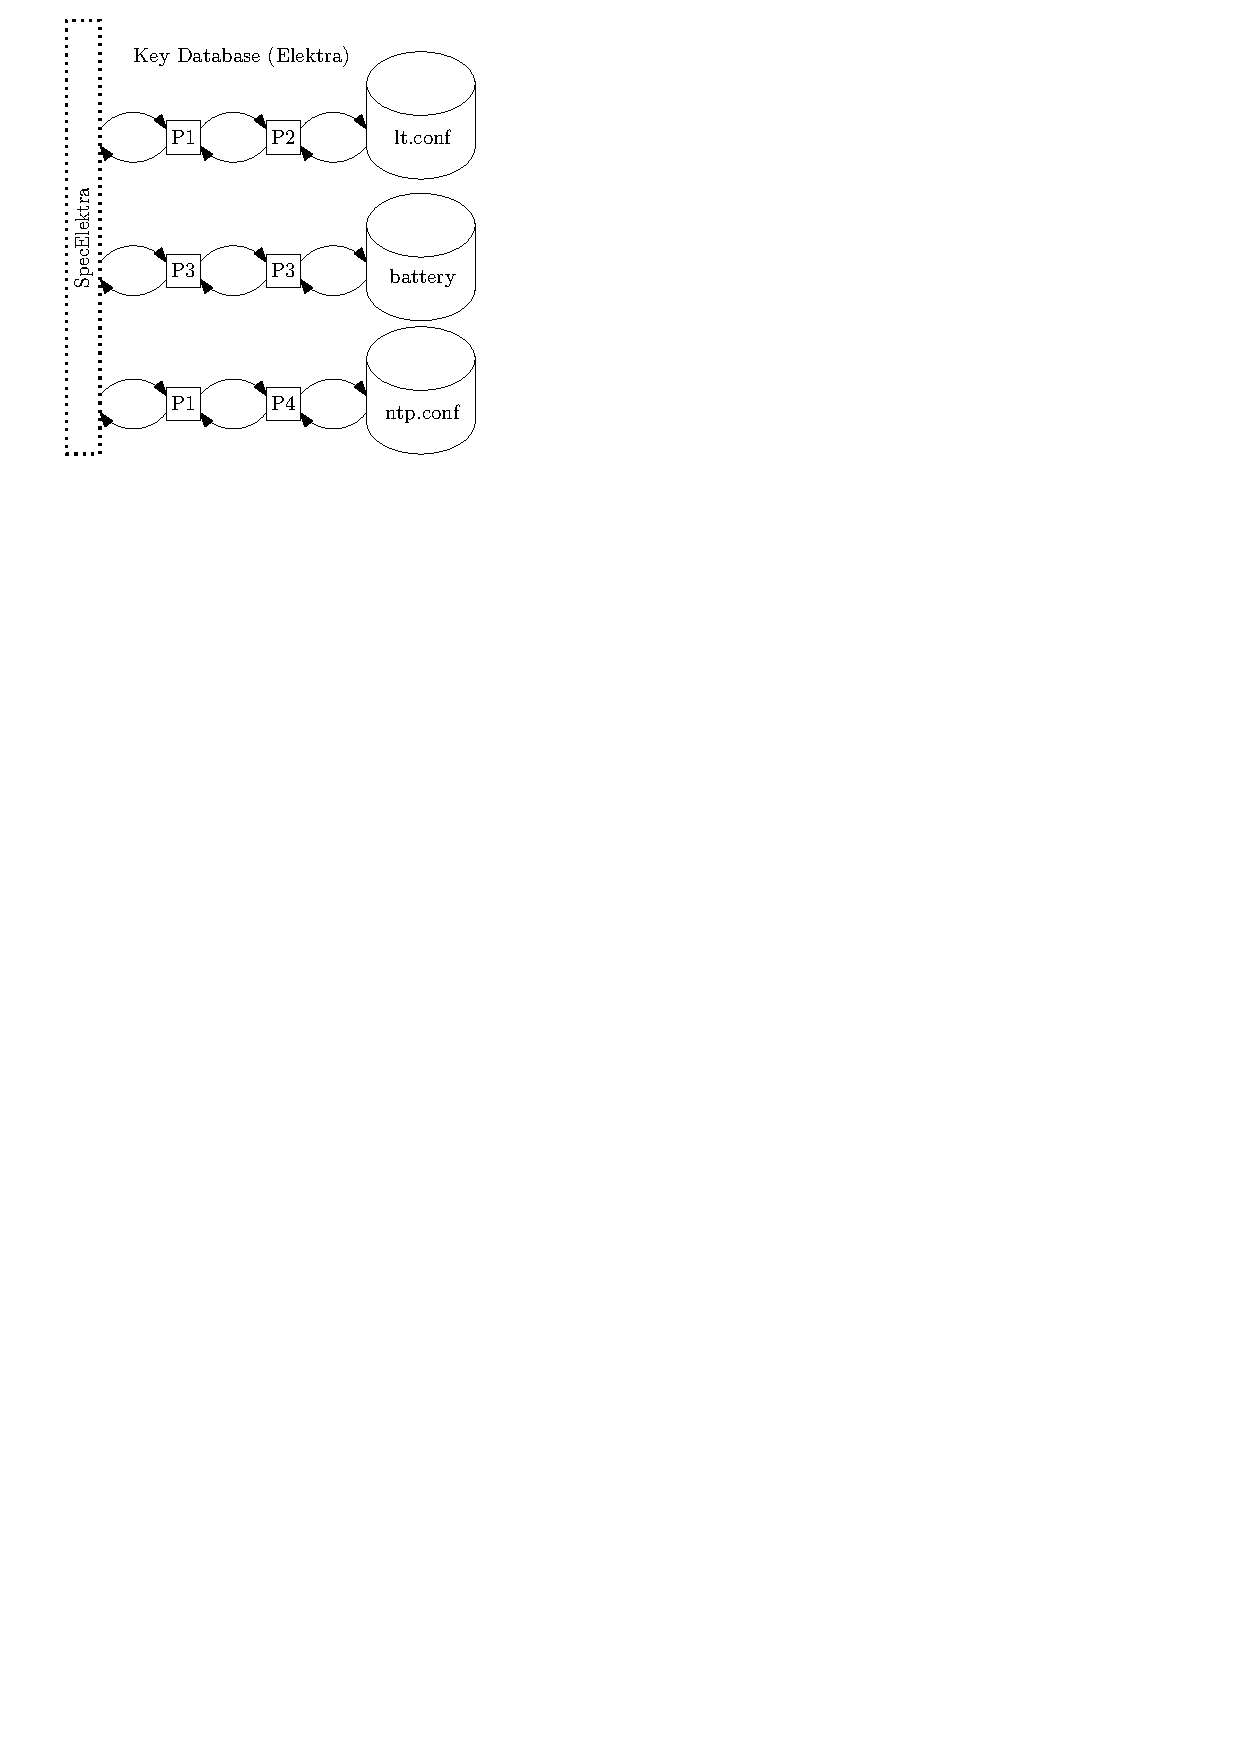
\includegraphics[scale=0.8]{horizontalmodularity}
	\end{column}
	\begin{column}{4cm}
	Cylinders are configuration files, P? are plugins~\cite{raab2016improving}.

	Key ideas:
	\begin{itemize}
	\item all work is done by plugins
	\item central data structure implements semantics
	\end{itemize}
	\end{column}
	\end{columns}
\end{frame}

\begin{frame}
	\frametitle{KeySet}

	The common data structure between plugins:
	\vspace{1cm}

	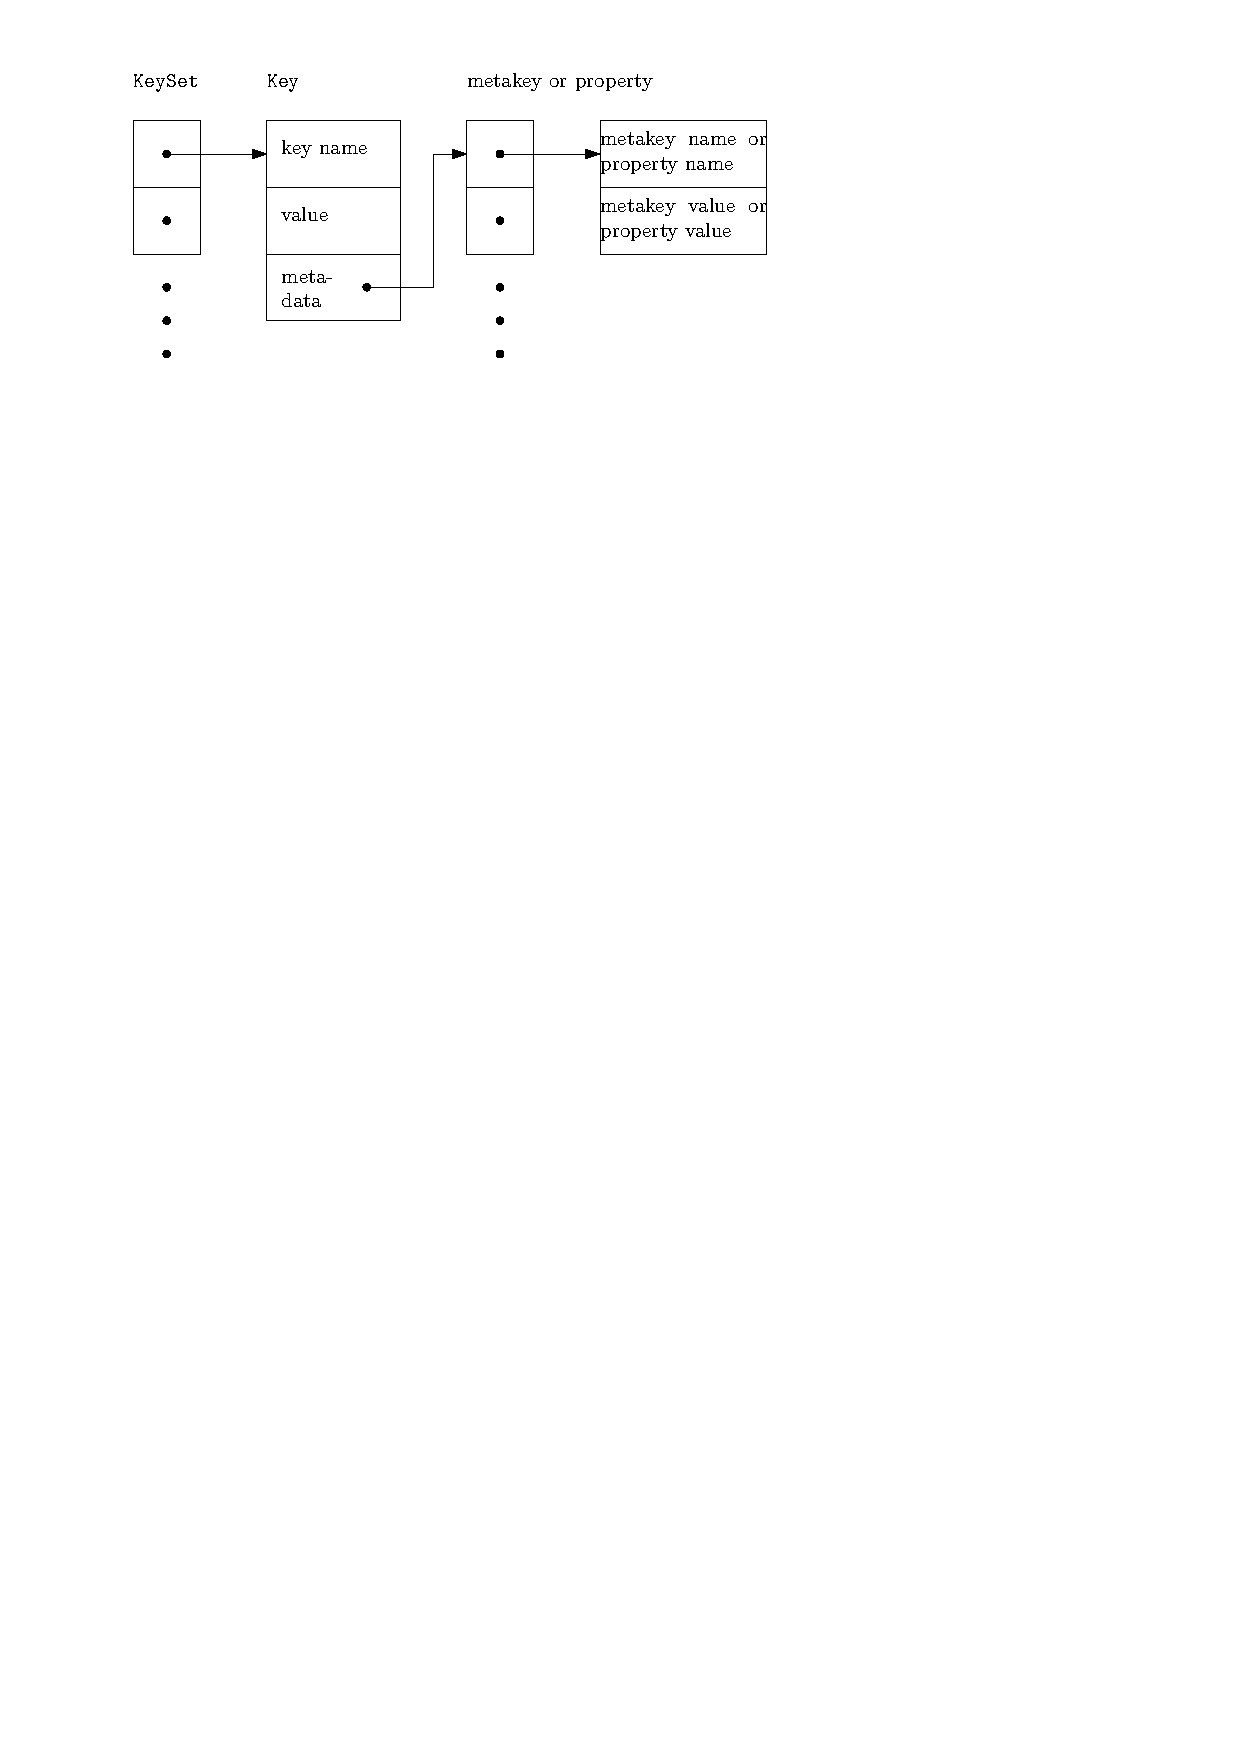
\includegraphics{keyset}
\end{frame}

\begin{assignment}
	\begin{task}
	Is meta-data separated from or included in the data structure?
	\end{task}
\end{assignment}

\begin{frame}[fragile]
	\begin{description}[align=left]
	\item[kdb.open():]
	The first step is to bootstrap into a situation where the necessary plugins can be loaded.
	\item[kdb.get(\texttt{KeySet}):] \index{kdb.get}
	The application (initially) fetches and (later) updates its configuration settings as a key set of type ^KeySet^ from the execution environment by one or many calls to ^kdb.get^.
	%If all relevant configuration files are unmodified since the last invocation, ^kdb.get^ will do nothing.
	\item[kdb.set(\texttt{KeySet}):] \index{kdb.set}
	When a user finishes editing configuration settings, ^kdb.set^ is in charge of writing all changes back to the key database.
	%This function atomically persists a whole key set in involved parts of the execution environment.
	%In the case of an error no action takes place.
	\item[kdb.close():] \index{kdb.close}
	The last step is to close the connection to the key database.
	\end{description}
\end{frame}

\begin{assignment}
	\begin{task}
	Break.
	\end{task}
\end{assignment}

\subsection{Metalevels}

\begin{frame}
	\frametitle{Metalevels}
	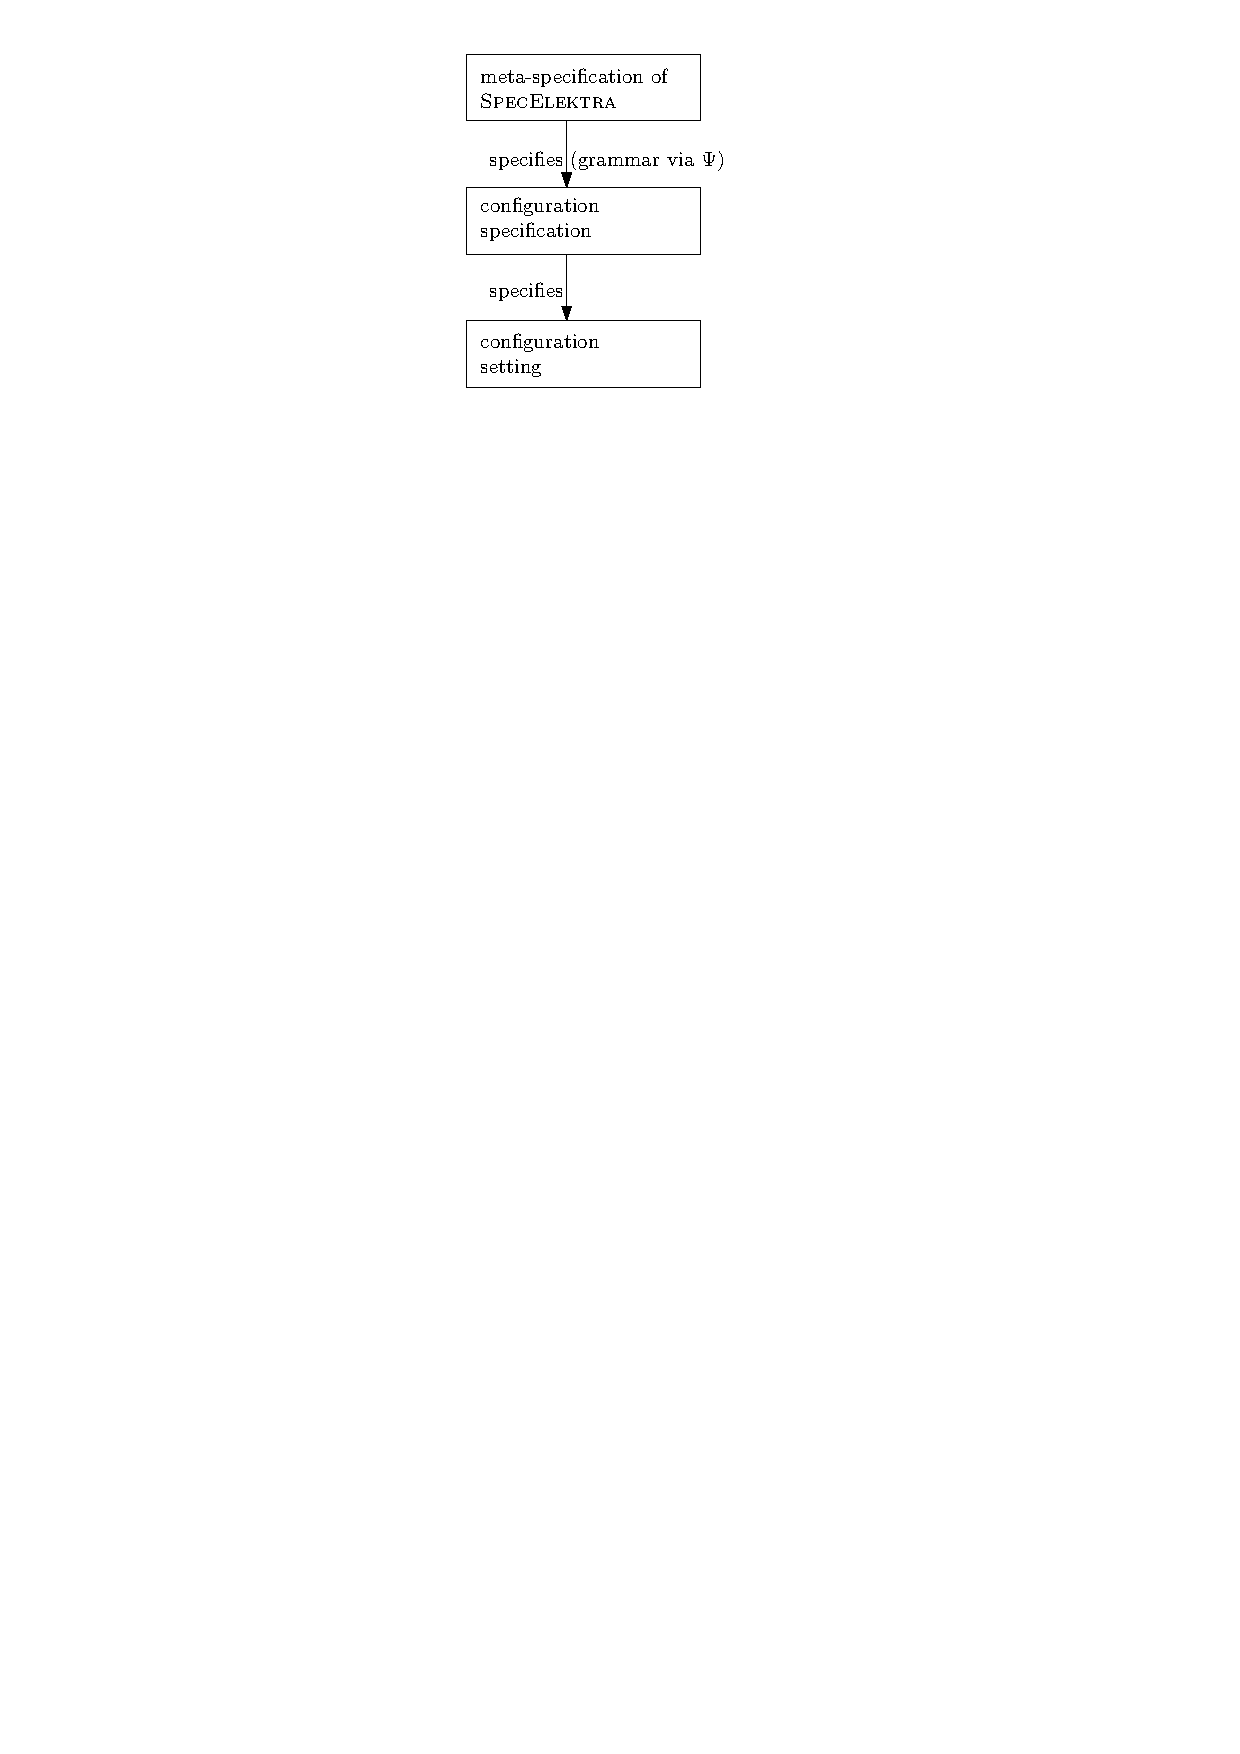
\includegraphics{metalevels}

	We will now walk through metalevels bottom-up.
\end{frame}

\begin{frame}[fragile]
	\frametitle{Configuration Settings}

	A configuration file may look like:

	\begin{code}[language=CfgElektra]
	a=5
	b=10
	c=15
	\end{code}

	We apply these configuration settings imperatively using:

	\begin{code}[language=bash]
	kdb set /a 5
	kdb set /b 10
	kdb set /c 15
	\end{code}

	And we list them with \lstinline[language=bash,morekeywords={ls},showspaces=no]^kdb ls /^.
\end{frame}

\begin{frame}[fragile]
	\frametitle{Specifications}
	For specifications such as:

	\begin{code}
	[slapd/threads/listener]
	  check/range:=1,2,4,8,16
	  default:=1
	\end{code}

	We apply the specifications imperatively using:

	\begin{code}[language=bash,morekeywords={meta-set}]
	kdb meta-set /slapd/threads/listener\
		check/range 1,2,4,8,16
	kdb meta-set /slapd/threads/listener\
	       	default 1
	\end{code}

	(automatically uses ^spec^ namespace)
\end{frame}

\begin{frame}[fragile]
	\frametitle{Meta-Specifications}
	For meta-specifications such as:

	\small
	\begin{code}
	[visibility]
	type:=enum critical important user\
	      advanced developer debug disabled
	description:=Who should see this\
	     configuration setting?
	\end{code}

	We apply the meta-specifications imperatively using:

	\begin{code}[language=bash,morekeywords={meta-set}]
	kdb meta-set /elektra/meta/\
		visibility type enum ...
	kdb meta-set /elektra/meta/\
		visibility description "Who ...
	\end{code}

	(see ^doc/METADATA.ini^, disclaimer: 1.0 not yet released)
\end{frame}

\begin{assignment}
	\begin{task}
	Brainstorming: Ideas for (meta-)specifications.
	\end{task}
\end{assignment}

\subsection{Conclusions}

\begin{frame}
	\frametitle{Introspection}
	\begin{itemize}[<+->]
	\item unified get/set access to (meta*)-key/values
	\item access via applications, CLI, GUI, web-UI, ...
	\item GUI, web-UI can semantically interpret metadata
	\item access via any programming language
	\item access via any configuration management system
	\end{itemize}
\end{frame}

\begin{frame}
	\frametitle{Users of Elektra}
	\begin{itemize}[<+->]
	\item Embedded systems
	\begin{itemize}
	\item OpenWRT (distribution)
	\item Broadcom (blue-ray devices)
	\item Kapsch (cameras)
	\item Toshiba (TVs)
	\end{itemize}
	\item Server
	\begin{itemize}
	\item Allianz (insurance)
	\item TU Wien
	\item puppet-libelektra
	\item Other Universities
	\end{itemize}
	\item Desktop
	\begin{itemize}
	\item Oyranos
	\item LCDproc (in progress)
	\item KDE
	\end{itemize}
	\end{itemize}
\end{frame}

\begin{frame}
	\frametitle{Conclusion}
	\begin{itemize}
	\item goals:
		\begin{itemize}
		\item make simple configuration management tasks simple
		\item improve robustness
		\item improve extensibility (reusable plugins operating on key/value)
		\item improve performance
		\item good defaults
		\item system-wide introspection
		\item system-level dependency injection
		\end{itemize}
	\item \elektra{} has no dependence to other libraries but only concrete plugins introduce dependences.
	\end{itemize}
\end{frame}




\appendix

\begin{frame}[allowframebreaks]
	\bibliographystyle{plainnat}
	\bibliography{../shared/elektra.bib}
\end{frame}

\end{document}

